\documentclass[conference]{IEEEtran}

\usepackage{svg}
\usepackage{amsmath,amssymb,amsfonts}

\usepackage{hyperref}
\usepackage{subcaption}
\usepackage{float}

\usepackage[english]{babel}
\usepackage{csquotes}
\usepackage[T1]{fontenc}

\usepackage[
    backend=biber,
    style=ieee
]{biblatex}
\addbibresource{bibliography.bib}

\usepackage[bb=dsserif]{mathalpha}

\usepackage{algorithmic}
\usepackage{graphicx}
\usepackage{textcomp}
\usepackage{xcolor}
    
\graphicspath{{img/}}
    
\begin{document}

\title{Makeup recommendation using machine learning and augmented reality}

\author{
\IEEEauthorblockN{Sebastian Pietras}
\IEEEauthorblockA{
\textit{Wydział Elektroniki i Technik Informacyjnych} \\
\textit{Politechnika Warszawska}\\
Warszawa, Polska \\
sebastian.pietras.stud@pw.edu.pl
}
\and
\IEEEauthorblockN{Maciej Konrad Kapuściński}
\IEEEauthorblockA{
\textit{Wydział Elektroniki i Technik Informacyjnych} \\
\textit{Politechnika Warszawska}\\
Warszawa, Polska \\
maciej.kapuscinski2.stud@pw.edu.pl
}
}

\maketitle

\begin{abstract}
Choosing the right makeup that matches a given face is a substantial task because the goal is to make one look more attractive. However, it is not easy, as learning the correct rules of makeup selection requires years of experience. In order to simplify that matter, this thesis presents a system capable of suggesting makeup based on facial features. With the help of machine learning techniques, a model was created that generates makeup color palettes. A mobile application was implemented that simulates the application of makeup on the face using augmented reality mechanisms. The system architecture, the implementation of its individual parts, and the obtained results were presented.
\end{abstract}

\section{Introduction} \label{sec:into}

Beauty is a positive aesthetic value.
It provides a sense of fulfillment and satisfaction.
For many people, beauty is a part of their identity.
Many people strive to look beautiful so that others will find them attractive.

Using makeup is one of the most common ways to boost one's beauty.
Makeup is a cosmetic product that is applied mainly to the face.
It can be used to hide blemishes, enhance features, or change the shape of the face.
There are many different types of makeup, including foundation, blush, eyeliner, mascara, and lipstick.

The art of applying makeup is not easy.
It requires a lot of practice and skill.
It can be challenging to know what colors and styles will look best on you.
It would be desirable to have a tool that could help you choose the best makeup for you.

This paper describes a system that uses machine learning and augmented reality to recommend makeup to users.
The system uses a machine learning model to predict the best makeup for a given user.
With the help of augmented reality, the system can show the user what the makeup will look like on them.
It is designed to be used by makeup artists, who can use it to help their clients choose the best makeup, or by casual users who want to find the best makeup for themselves.

\section{Related Work} \label{sec:related}

There have been a number of attempts to create various types of makeup recommendation systems.
In \cite{scherbaum2011computer}, a database of 3D scans of faces before and after makeup application was collected.
To suggest makeup to users, the system searches the database for faces that are similar to the user's face and applies the associated makeup.
The solution has a high visual quality, but it is limited to the makeup that is already in the database.

In \cite{alashkar2017rule}, a solution was proposed that uses an algorithm based on well-known makeup rules.
Face images are analyzed to determine the facial features, and then the makeup is applied based on the rules concerning the features.
The drawback of this solution is that it is limited to well-defined makeup rules that need to be provided by a makeup expert.

Quite a different approach was presented in \cite{shreyank2019using}.
A neural network was trained to colorize black-and-white images of faces.
The network was trained on a dataset of faces with makeup applied.
This way, the network learned to colorize faces as if they were wearing makeup.
The problem with this solution is that the input images need to be black-and-white, which results in a considerable loss of important information.

\section{Representation} \label{sec:representation}

The goal of the system is to recommend makeup based on facial features.
Both the makeup and the facial features need to be represented in a way that is suitable for processing by a machine-learning model.

\subsection{Makeup}

Makeup consists of various types of cosmetics, such as foundation, blush, eyeliner, mascara, and lipstick.
In order to keep the system relatively simple, only lipstick and eyeshadow are considered.
The reason for this is these are the most outstanding elements of makeup.

In the system, the lipstick is represented by a single color, applied evenly to the entire lips.
On the other hand, eyeshadow is represented by three colors, applied to the area around the eyes as a gradient from the inner eye corner to the outer eye corner.
All colors are represented in the LAB color space to make the distances between colors more similar to the distances that humans perceive \cite{tkalcic2003colorspaces}.

\subsection{Facial Features}

The facial features that are used in the system are skin color, eye color, lips color, and hair color.
All of them are represented by a single color in the LAB color space.

\section{Data} \label{sec:data}

In order to gain knowledge about makeup rules, a proper dataset is needed.
The most preferable one would be a dataset of faces before and after the makeup application.
We have not been able to find such a dataset, so we decided to modify another dataset to suit our needs.
The dataset that we used is the \emph{YouMakeup} dataset \cite{wang2019youmakeup}.
It contains about two thousand instructional videos of makeup application.
Most videos are available in high quality.
In addition, the dataset also contains metadata with timestamps of the start and end of each makeup step.
The people in the videos are from more than a hundred different \emph{YouTube} channels and represent many different beauty styles.
From the videos, we extracted the frames with faces before and after the makeup application.
Then, we extracted the facial features and the makeup from the frames.

\subsection{Preprocessing}

In order to extract the frames, it is necessary to find those frames where the face is most visible.
To do this, we used the face detection algorithm from the \emph{OpenCV} library \cite{opencv}.
Only frames within a few seconds around the start and end of the makeup application were considered.
Those frames for which the detection confidence value was the highest were selected.
In effect, one frame before and one frame after the makeup application were obtained from a single video.

About 600 videos were processed in this way.
In the remaining videos, the face was not detected at all.
The rest of the videos were manually inspected and this way we were able to extract frames from about 300 more videos.
This yielded a total of 975 pairs of frames before and after makeup application.

\subsection{Facial Features Extraction}

The frames before makeup application needed to be transformed into facial features.
To do this, we first used a \emph{MTCNN} face detector \cite{MTCNN-Zhang} to find a bounding box around the face.
Then, we used the \emph{BiSeNet} \cite{BiSeNet} segmentation model to segment the face into different parts, corresponding to the needed facial features.
The skin color, the lips color, and the hair color were calculated as a geometric median of all pixels in the corresponding part of the face.

The eye color was extracted in a slightly different way.
Eye color actually means the color of the iris, not the whole eye.
Because of that, we needed to reduce the considered area to the iris only.
As the color does not need to be strictly accurate, we decided to use a simple method to extract the iris.
We used the fact that the iris is darker than the surrounding area, but not as dark as the pupil.
We chose to remove $50\%$ of the brightest and $10\%$ of the darkest pixels from the eye area, roughly corresponding to the usual sizes of the sclera and the pupil.
Then, we calculated the geometric median of the remaining pixels.

\subsection{Makeup Extraction}

The frames after the makeup application needed to be transformed into makeup features.
To do this, we used the same \emph{MTCNN} face detector and \emph{BiSeNet} segmentation model as for the facial features extraction.
The lipstick was extracted as a geometric median of all pixels in the lips part of the face.

The extraction of the eyeshadow was somewhat more complicated.
Having the area of the eye, we enlarged it two times using a dilation operation.
We used an elliptical kernel with sizes $r_A \times r_A$ and $r_B \times r_B$, where $r_A$ is:
\begin{equation}
    r_A = \max{\left(\left\lfloor2{,}25\sqrt{P}\right\rfloor, 2\right)},
\end{equation}
and $r_B$ is:
\begin{equation}
    r_B = \max{\left(\left\lfloor0{,}25\sqrt{P}\right\rfloor, 1\right)},
\end{equation}
where $P$ is the number of pixels in the eye area.
Then, we subtracted the smaller area from the larger one, leaving only the area around the eye.
To make things safer, the final area was produced from the intersection of the resulting area and the area of the skin.

The resulting area should also include the eyelashes and unpainted skin.
These are not part of the eyeshadow, so they need to be removed.
To do this, we used a clustering algorithm to divide the area into clusters of pixels, assuming that two of the clusters correspond to the eyelashes and the unpainted skin.
We used agglomerative clustering with six clusters and average linkage.
The color of the skin is known from the facial features extraction and the color of the eyelashes is the darkest.
We used the $kNN$ algorithm with $k = 3$ to find the two clusters matching these colors.
Then, we removed the pixels from the resulting area that belongs to these clusters.

The remaining area is the eyeshadow.
To extract the colors, we needed to divide the area into three parts.
For this purpose, we used the $k$-means algorithm with $k = 3$ to find the three clusters of pixels.
The colors extracted from the clusters were used as the three colors of the eyeshadow.

\section{Model} \label{sec:model}

The task of the system is to find the best makeup for a given face.
To do this, we need to create a model that can predict the makeup for a given face.
More specifically, the model needs to predict the makeup features for given facial features.
Moreover, there might be more than one makeup suitable for a given face, so the model needs to consider this.

\subsection{Model Structure}

The model used in the system is one that can be classified as a Wasserstein Conditional Generative Adversarial Network (WCGAN) \cite{arjovsky2017wasserstein}.
The model consists of two parts, a generator, and a discriminator.
The generator is responsible for generating the makeup features for given facial features.
The discriminator is responsible for determining whether the makeup features are real or fake.
The generator is trained to fool the discriminator, while the discriminator is trained to distinguish between real and fake makeup features.
Facial features are used as a condition, passed to both the generator and the discriminator.
The Wasserstein version of the GAN is used to avoid the vanishing gradient problem.

We used simple multi-layer perceptrons as the generator and the discriminator.
To make the training as stable as possible, both networks should be of similar complexity.
The discriminator might be slightly more complex to make it more difficult for the generator to fool it before it is able to separate real and fake makeup features well.
On the other hand, it should not be too complex, because the generator needs to be able to fool it at some point.

The exact structure of the networks is as follows:

\begin{itemize}
    \item generator - $L^{24}_{18}$ $R_{0.01}$ $L^{18}_{12}$,
    \item discriminator - $L^{24}_{18}$ $R_{0.01}$ $D_{0.05}$ $L^{18}_{12}$ $R_{0.01}$ $D_{0.05}$ $L^{12}_{6}$ $R_{0.01}$ $D_{0.05}$ $L^{6}_{1}$.
\end{itemize}

In this notation, consecutive items are successive layers of the network, where:

\begin{itemize}
    \item $L^{a}_{b}$ - fully connected layer with $a$ inputs and $b$ outputs,
    \item $R_{\alpha}$ - \emph{LeakyReLU} activation function with a slope of $\alpha$ \cite{maas13relu},
    \item $D_{p}$ - \emph{Dropout} with a probability of $p$ \cite{dropout}.
\end{itemize}

\subsection{Training}

We used the \emph{Adam} optimizer \cite{kingma2017adam} to train the networks.
The learning rate for the generator was set to $0.0001$ and the learning rate for the discriminator was set to $0.001$.
Smaller learning rates were used for the generator to force it to take less radical steps when trying to fool the discriminator, which makes the training more stable.
The batch size was set to $128$ and the training was done for $500$ epochs.
The loss function used was the Wasserstein loss function with gradient penalty \cite{gulrajani2017improved}.

\begin{figure}
    \centering \includesvg[inkscapelatex=false,height=58mm]{loss_curve.svg}
    \vspace{2mm}
    \caption{Loss curve}
    \label{fig:loss_curve}
\end{figure}

The loss curve with mean loss value in each epoch is shown in Figure \ref{fig:loss_curve}.
If the loss value is close to zero, it means that the generator is able to fool the discriminator.
In the first epochs, you can see that the loss value decreases rapidly.
This is because the discriminator was able to learn to distinguish between real and fake makeup features quite quickly.
However, it is not perfect and the generator is able to take advantage of this in the next epochs.
The generated data starts to look more and more like real data and the loss value starts to get closer to zero.
In the end, an equilibrium is reached and the loss value stays around zero.
Neither the generator nor the discriminator is able to improve the situation.

\section{Visualisation} \label{sec:visualisation}

The system is able to visualize how the generated makeup features look on a given face on the user's device.
To be able to do this, we need a method that tracks the facial features in real-time.
The tracking should be fast enough to be able to run on the user's device.
Fortunately, Android provides a library that can be used for this purpose, called \emph{ML Kit} \cite{mlkit}.

The facial features that are needed are the eyes which are used to determine the position of the eyeshadow and the lips which are used to determine the position of the lipstick.
We use the key points provided by the library and connect them with Bezier curves to get the areas of the eyes and the lips.
In the case of the lips, this is all that is needed.
However, in the case of the eyes, we need to get the area around the eyes.
To do this, we use a ready-made eyeshadow shape, which we place where the eyes are.
Then, we scale it relative to the width of the eye and the distance between the center of the eye and the center of the eyebrow.

After calculating the needed areas and getting the colors of the makeup features from the model, we can start drawing the makeup on the face.
The makeup features are drawn on the face inside the areas calculated earlier.
The lipstick is drawn on the lips area evenly.
The eyeshadow is drawn on the eyeshadow area as a gradient from ranging one corner of the eye to the other.
We use blending to make the colors look smooth and natural.
The parameters of the blending were determined experimentally.

\section{Architecture} \label{sec:architecture}

The system consists of two parts, the server, and the client.
The architecture of the system is shown in Figure \ref{fig:architecture}.

\begin{figure}
    \centering \includesvg[inkscapelatex=false,height=58mm]{architecture.svg}
    \vspace{2mm}
    \caption{Architecture diagram}
    \label{fig:architecture}
\end{figure}

\subsection{Server}

The server is responsible for generating the makeup features for given facial features.
It gets the picture of the face from the client.
Then, it extracts the facial features from the picture in the same way as described in the \ref{sec:data} section.
The facial features are then passed to the model to generate the makeup features.
Then, the makeup features are sent back to the client.

The server is implemented in \emph{Python} using the \emph{Flask} framework \cite{flask}.
The model is implemented using the \emph{PyTorch} framework \cite{pytorch}.
The pictures are sent to the server as files and the makeup features are sent as JSON objects over HTTP.

\subsection{Client}

The client is responsible for sending the picture of the face to the server and displaying the makeup features.
The user takes a picture of the face using the camera.
The picture is then sent to the server.
The returned makeup features are then used to display the makeup on the face.

The client is implemented in \emph{Kotlin} and \emph{Java} as an \emph{Android} application.
The camera is accessed using the \emph{CameraX} library \cite{CameraX}.
The HTTP requests are sent using the \emph{OkHttp} library \cite{OkHttp}.
Face detection is done using the \emph{ML Kit} library \cite{mlkit}.

\section{Results} \label{sec:results}

The final working system is able to generate and visualize makeup that is suitable for a given face. An example of the generated makeup is shown in Figure \ref{fig:example}.

\begin{figure}
    \centering
    \begin{subfigure}{0.49\linewidth}
        \centering 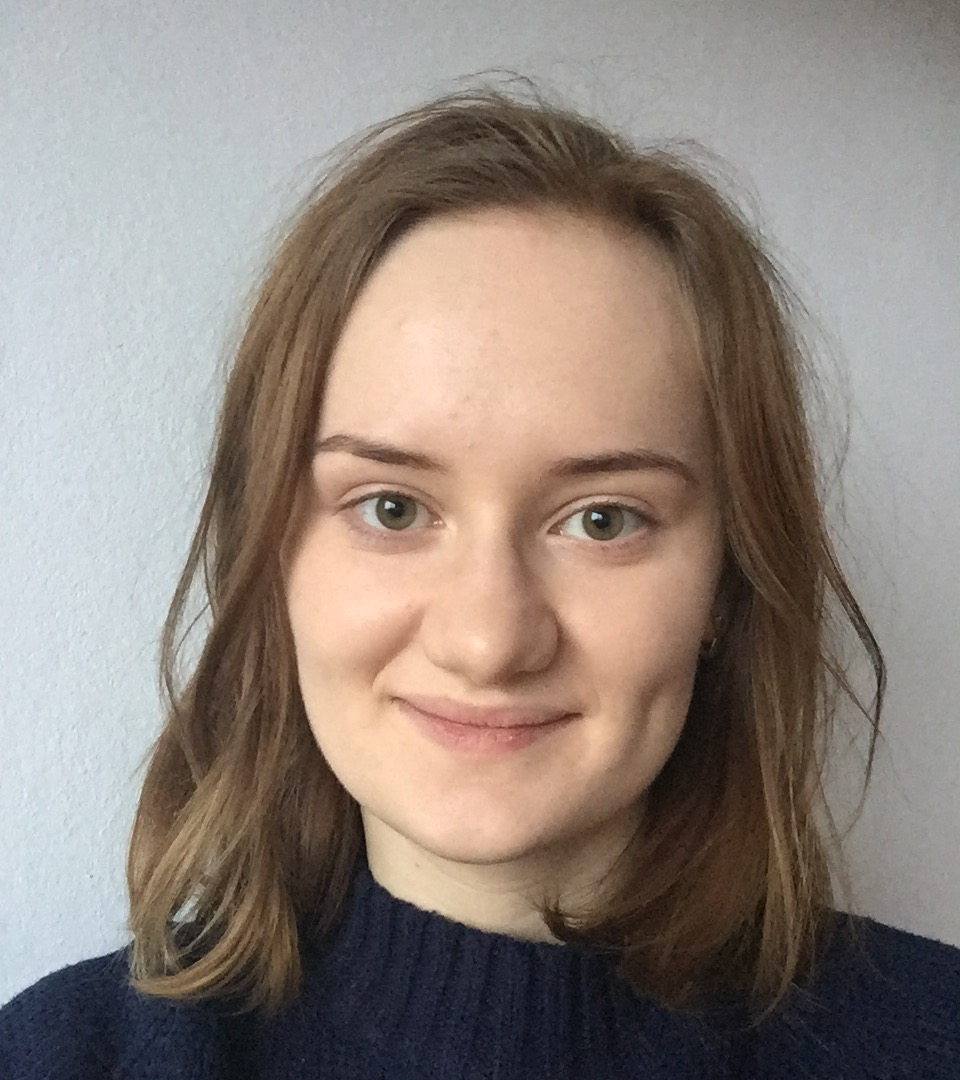
\includegraphics[height=9\baselineskip]{before.png}
        \caption{Before applying makeup}
    \end{subfigure}
    \hfill
    \begin{subfigure}{0.49\linewidth}
        \centering 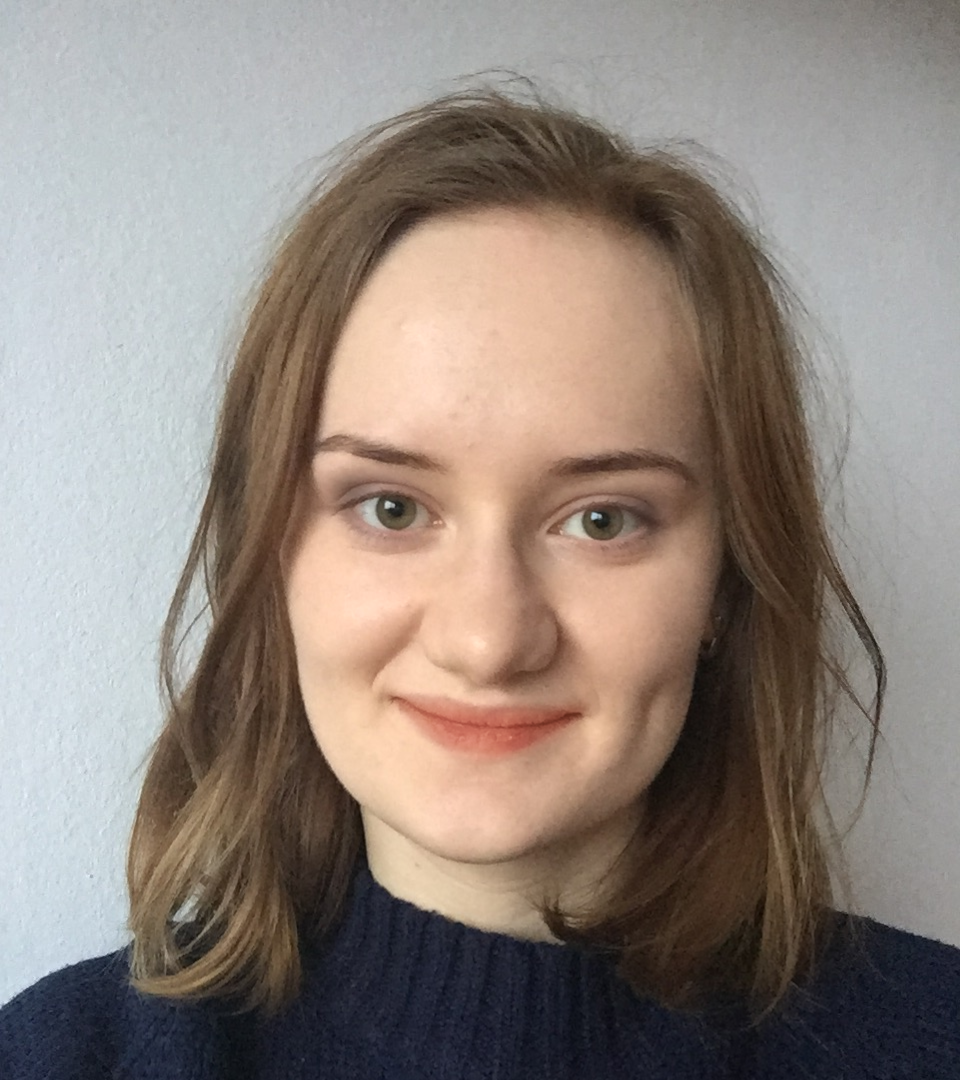
\includegraphics[height=9\baselineskip]{after.png}
        \caption{After applying makeup}
    \end{subfigure}
    \par\vspace{0.5\baselineskip}
    \begin{subfigure}{0.49\linewidth}
        \centering \includesvg[inkscapelatex=false,height=3\baselineskip]{face_features.svg}
        \caption{Facial features}
    \end{subfigure}
    \hfill
    \begin{subfigure}{0.49\linewidth}
        \centering \includesvg[inkscapelatex=false,height=3\baselineskip]{makeup_features.svg}
        \caption{Makeup features}
    \end{subfigure}
  \caption{Example of applied generated makeup}
  \label{fig:example}
\end{figure}

In order to evaluate the quality of the generated makeup, we made a survey.
It consisted of $10$ questions, each with a picture of a face before applying makeup and $5$ makeup color palettes.
One of the palettes was the real makeup that was applied to the face and the other four were generated by the system.
The participants were asked to order the palettes from the most suitable to the least suitable.
The survey was answered by $25$ people from various Internet beauty communities.

\begin{figure}
    \vspace{0.1\baselineskip}
    \centering \includesvg[inkscapelatex=false,height=14\baselineskip]{survey.svg}
    \vspace{0.1\baselineskip}
    \caption{Histogram of the positions of the real makeup palette}
    \label{fig:survey}
\end{figure}

The histogram of the positions of the real makeup palette is shown in Figure \ref{fig:survey}.
The first four positions are fairly evenly distributed, which means that the system is able to generate makeup that is at least as good as the real one.
Surprisingly, the last position is the most frequent one, which means that the real makeup was often considered the least suitable.
This might be because the generated palettes were often more colorful than the real ones, which might get people's attention.
The presented results suggest that the system is able to generate makeup that is likely to be considered good enough by the users.

\section{Conclusion} \label{sec:conclusion}

The implemented system enables users to easily try out different makeup styles on their faces.
The generated makeup is based on the facial features of the user and is therefore likely to be suitable for the user.
The visualization of the generated makeup is also very useful because it allows the user to see how the makeup looks on the face.
The conducted survey suggests that the generated makeup is at least as good as a real one.

Multiple improvements can be made to the system.
The first one is to extend the representation of facial features.
More features can be extracted from the face, which might have a significant influence on which makeup is suitable for the user.
The second one is to increase the complexity of the generated makeup.
It could include more elements, such as eyeliner, eyebrows, etc.
The third one is to collect more data for the model with a wider variety of makeup styles.
The next one is to improve the visualization of the generated makeup as the current one is not the most accurate.


\printbibliography

\end{document}
